\chapter{Counting intersections of curves}
\section{Where curves intersect}
\epigraph[author={Chico Marx}]{Who are you going to believe, me or your own eyes?}\SubIndex{Marx, Chico}
\begin{example}
A line through a cubic curve
\begin{center}
\inputinexample{cubic-curve-4}
\end{center}
can hit as many as \(3\) points.
\end{example}
\begin{example}
Two conics
\begin{center}
\newcommand{\conicshift}{-.5}
\inputinexample{2-conics}
\end{center}
can intersect at as many as \(4\) points, but sometimes only at \(3\) points:
\begin{center}
\newcommand{\conicshift}{.875}
\inputinexample{2-conics}
\end{center}
\end{example}
\begin{example}
Some conics don't appear to intersect at all
\begin{center}
\newcommand{\conicshift}{4}
\inputinexample{2-conics}
\end{center}
but keep in mind that our points can have coordinates in the algebraic closure, so they actually intersect.
\end{example}
\begin{example}
The conics \(x^2+y^2=1\) and \((x-4)^2+y^2=1\):
\inputinexample{unnested-circles}
intersect at \((x,y)=(2,\pm i \sqrt{3})\). 
\end{example}
\begin{example}
Some conics appear not to have even complex intersections, such as \(x^2+y^2=1\) and \(x^2+y^2=2\).
\inputinexample{nested-circle}
But in the projective plane, we can homogenise to \(x^2+y^2=z^2\) and \(x^2+y^2=2z^2\), and then intersect with the plane \(x=1\), to get \(1+y^2=z^2\) and \(1+y^2=2z^2\), which intersect at \((y,z)=(\pm i,0)\).
\end{example}
\begin{problem}{intersecting.curves:irred.inter}
Take integers \(m,n\ge 2\).
Over any field of characteristic zero, prove that the plane algebraic curves \(B=(y=x^m)\) and \(C=(x+1=y^n)\) intersect at \(mn\) distinct points in the affine plane, and no points on the line at infinity.
Prove that these curves are irreducible.
\end{problem}
\begin{answer}{intersecting.curves:irred.inter}
Take resultant
\begin{align*}
r(x)
&=
\det
\begin{pmatrix}
-x^m & 0  & \dots & \dots & 0 & -(x+1) \\
    1&-x^m& 0     & \dots & 0 & 0 \\
     &   1& -x^m  & \dots & 0 & 0 \\
     &    & \ddots& \ddots & \vdots & \vdots \\
     &    &       & 1      & -x^m & 0 \\
     &    &       &        &  1 & 1           
\end{pmatrix},\\
&=
-x^m
\det
\begin{pmatrix}
-x^m& 0     & \dots & 0 & 0 \\
   1& -x^m  & \dots & 0 & 0 \\
    & \ddots& \ddots & \vdots & \vdots \\
    &       & 1      & -x^m & 0 \\
    &       &        &  1 & 1           
\end{pmatrix}\\
&\quad+
(-1)^n(-(x+1))
\det
\begin{pmatrix}
    1&-x^m& 0     & \dots & 0 \\
     &   1& -x^m  & \dots & 0 \\
     &    & \ddots& \ddots & \vdots \\
     &    &       & 1      & -x^m \\
     &    &       &        &  1           
\end{pmatrix},\\
&=
(-1)^n(x^m-x-1)).
\end{align*}
To have a double root or higher, we need \(x^m=x+1\), and also vanishing of the derivative \(mx^{m-1}=1\), so \(x^m=x/m=x+1\), so \(x=m/(m-1)\) is rational, so lies inside the rational numbers in our field.
But then we need \(x^{m-1}=1/m\), so \(m^m=(m-1)^{m-1}\), clearly impossible in usual rational numbers because \(m>m-1\) so \(m^m>(m-1)^{m-1}\).
So our resultant has only single roots, i.e. intersections arise at only one point each.
The reader can prove that the curves are irreducible.
The curves reach the line at infinity at \(0=x^m\) and \(0=y^n\), i.e \([x,y,z]=[0,1,0]\) and \([x,y,z]=[1,0,0]\), so not intersection points at infinity.
\end{answer}
\begin{problem}{projective.curves:do.intersect}
Prove that any two plane algebraic curves intersect in the projective plane.
\end{problem}
\begin{answer}{projective.curves:do.intersect}
Homogenize their equations.
Proposition~\vref{proposition:resultant.degree} shows that either they have a common component or the equations have nonzero resultant, a homogeneous polynomial of degree
exactly the product of their degrees, say \(m\) and \(n\).
After a shearing, we can arrange that the resultant has highest terms with nonzero pure power \(x^{mn}\).
Dehomogenize by setting \(x=1\).
The degree of the resultant doesn't go down, so is positive.
The curves now intersect, after some finite field extension to introduce roots to the resultant.
\end{answer}
\begin{problem}{counting.intersections:finiteness}
Prove that any two plane algebraic curves sharing no component have finitely many intersections in the projective plane.
\end{problem}
\begin{answer}{counting.intersections:finiteness}
There are finitely many intersection points of \(B\) and \(C\) in the affine \(xy\)-plane by corollary~\vref{corollary:finite.intersection}.
There are finitely many more on the line at infinity by lemma~\vref{lemma:one.variable.splits.3}. 
\end{answer}
\begin{problem}{projective.curves:finite.image}
Suppose that \(f\colon B\to\Proj^n\) is a rational morphism of a curve, with image contained in a finite set of points.
Then \(f\) is constant.
\end{problem}
\begin{answer}{projective.curves:finite.image}
We can assume, perhaps after a finite field extension and a projective automorphism, that none of these finitely many points is at infinity.
For simplicity of notation, we only prove the case of \(n=2\), i.e. rational morphisms to the projective plane, say
\[
(X,Y)=f(x,y)=(X(x,y),Y(x,y)),
\]
with rational functions \(X=X(x,y), Y=Y(x,y)\), mapping to the affine plane.
First suppose that \(B\) is irreducible.
Suppose that \(f\) maps to some points \((X,Y)=(X_1,Y_1),\dots,(X_n,Y_n)\).
The polynomial \(p(X,Y)=(X-X_1)\dots(X-X_n)\) vanishes on these points, so \(p\circ f=0\), i.e. the rational function
\[
p(X(x,y),Y(x,y))
\]
vanishes, so its numerator vanishes.
It is a product of the rational functions 
\[
X(x,y)-X_1, X(x,y)-X_2,\dots,X(x,y)-X_n,
\]
so the numerator of at least one of these vanishes, i.e \(X(x,y)\) is constant.
Similarly for \(Y(x,y)\).
Next suppose that \(B\) is reducible.
So our map is constant on each component of \(B\), and hence regular everywhere.
Any two components meet by problem~\vref{problem:projective.curves:do.intersect}.
Our map is regular at the intersection points, so the constants agree.
\end{answer}

\section{Counting intersections}
In the projective plane, we have a concept of line, but not of line segment, or of angle or distance.
In a projective plane a \emph{triangle}\define{triangle} \(pqr\) is a triple of points \(p,q,r\) not all on the same line, together with the lines that connect them.
So a triangle looks like
\[
\begin{tikzpicture}
\clip (-1/3,-2/3) rectangle (4/3,2/3);
\draw[very thick,curveZero] (-1/3,-1/6) -- (4/3,2/3);
\draw[very thick,curveZero] (-1/3,7/3) -- (4/3,-1);
\draw[very thick,curveZero] (-1/3,1/9) -- (4/3,-4/9);
\end{tikzpicture}
\]
rather than
\[
\begin{tikzpicture}
\draw[very thick,curveZero] (0,0) -- (2/3,1/3) -- (1,-1/3) -- cycle;
\end{tikzpicture}
\]
A triangle \(pqr\) is \emph{generic}\define{generic!triangle}\define{triangle!generic} for two plane algebraic curves \(B, C\) if 
\begin{enumerate}
\item
neither curve passes through \(q\) and
\item 
no line connecting two intersection points of \(B\) and \(C\) lies through \(q\).
\end{enumerate}
\begin{center}
\documentclass[tikz]{standalone}
\usetikzlibrary{intersections}
\usepackage{xparse}
\colorlet{curveZero}{gray!85}
\colorlet{curveOne}{blue!60}
\definecolor{curveOneColor}{rgb}{.6,0,0}
\colorlet{curveTwo}{brown!50!gray}
\colorlet{curveThree}{green!40!gray}
\colorlet{curveFour}{red!50!gray}
\NewDocumentCommand\DrawDotInPlot{O{}mmO{}}%
{%
\fill[gray!15,draw=gray] (axis cs:{#2},{#3}) circle [radius=1.6pt] node[above,black,#4] {\(#1\)};%
}%
\NewDocumentCommand\DrawDot{O{}mmO{}}%
{%
\fill[gray!20,draw=gray] ({#2},{#3}) circle (1.6pt) node[above,black,#4] {\(#1\)};%
}%
\NewDocumentCommand\DrawNode{O{}m}%
{%
\fill[gray!20,draw=gray] (#2) circle (1.6pt) node[above,black] {\(#1\)};%
}%
\NewDocumentCommand\DrawDotThreeD{O{}mmmO{}}%
{%
\fill[gray!20,draw=gray] ({#2},{#3},{#4}) circle (1.6pt) node[above,black,#5] {\(#1\)};%
}%
\colorlet{axisColor}{gray!50}
\tikzstyle{shapeZero}=[fill=curveZero,opacity=.4]
\tikzstyle{shapeOne}=[fill=curveOne,opacity=.4]
\tikzstyle{shapeTwo}=[fill=curveTwo,opacity=.4]
\tikzstyle{shapeThree}=[fill=curveThree,opacity=.4]
\tikzstyle{groupElementLabel}=[minimum size=2.4em]
\tikzstyle{groupElement}=[minimum size=2.4em,shapeZero,draw=curveZero]
\tikzstyle{cosetOne}=[minimum size=2.4em,shapeOne,draw=curveOne]
\tikzstyle{cosetTwo}=[minimum size=2.4em,shapeTwo,draw=curveTwo]


\begin{document}
\begin{tikzpicture}[scale=3]
\draw[curveZero,very thick] 
({cos(90)},{sin(90)}) node[black,above] {\(q\)} -- 
({cos(90+120)},{sin(90+120)}) node[black,below left] {\(p\)} -- 
({cos(90+2*120)},{sin(90+2*120)}) node[black,below right] {\(r\)} -- cycle;
\draw[curveOne,name path=Bellipse,very thick] ({.5*cos(90)+.5*cos(90+2*120)},{.5*sin(90)+.5*sin(90+2*120)}) arc (30:390:.45);
\draw[curveTwo,name path=Cellipse,very thick] ({.5*cos(90)+.5*cos(90+2*120)},{.5*sin(90)+.5*sin(90+2*120)}) arc (30:390:.3 and .6);
\draw [axisColor, name intersections={of=Bellipse and Cellipse}]
(intersection-1) -- ({cos(90)},{sin(90)}) 
(intersection-2) -- ({cos(90)},{sin(90)}) 
(intersection-3) -- ({cos(90)},{sin(90)}) 
(intersection-4) -- ({cos(90)},{sin(90)}); 
\end{tikzpicture}
\end{document}

\end{center}
The triangle is \emph{very generic}\define{very generic!triangle}\define{triangle!very generic}
\define{generic!triangle!very} if it is generic and there is no intersection point of \(B\) and \(C\) along the line \(qr\).
Keep in mind that we allow intersection points, and points of the triangle, to have coordinates in the algebraic closure of our field.
\begin{center}
\documentclass[tikz]{standalone}
\usetikzlibrary{intersections}
\usepackage{xparse}
\colorlet{curveZero}{gray!85}
\colorlet{curveOne}{blue!60}
\definecolor{curveOneColor}{rgb}{.6,0,0}
\colorlet{curveTwo}{brown!50!gray}
\colorlet{curveThree}{green!40!gray}
\colorlet{curveFour}{red!50!gray}
\NewDocumentCommand\DrawDotInPlot{O{}mmO{}}%
{%
\fill[gray!15,draw=gray] (axis cs:{#2},{#3}) circle [radius=1.6pt] node[above,black,#4] {\(#1\)};%
}%
\NewDocumentCommand\DrawDot{O{}mmO{}}%
{%
\fill[gray!20,draw=gray] ({#2},{#3}) circle (1.6pt) node[above,black,#4] {\(#1\)};%
}%
\NewDocumentCommand\DrawNode{O{}m}%
{%
\fill[gray!20,draw=gray] (#2) circle (1.6pt) node[above,black] {\(#1\)};%
}%
\NewDocumentCommand\DrawDotThreeD{O{}mmmO{}}%
{%
\fill[gray!20,draw=gray] ({#2},{#3},{#4}) circle (1.6pt) node[above,black,#5] {\(#1\)};%
}%
\colorlet{axisColor}{gray!50}
\tikzstyle{shapeZero}=[fill=curveZero,opacity=.4]
\tikzstyle{shapeOne}=[fill=curveOne,opacity=.4]
\tikzstyle{shapeTwo}=[fill=curveTwo,opacity=.4]
\tikzstyle{shapeThree}=[fill=curveThree,opacity=.4]
\tikzstyle{groupElementLabel}=[minimum size=2.4em]
\tikzstyle{groupElement}=[minimum size=2.4em,shapeZero,draw=curveZero]
\tikzstyle{cosetOne}=[minimum size=2.4em,shapeOne,draw=curveOne]
\tikzstyle{cosetTwo}=[minimum size=2.4em,shapeTwo,draw=curveTwo]


\begin{document}
\begin{tikzpicture}[scale=3]
\draw[curveZero,very thick] 
({cos(90)},{sin(90)}) -- 
({cos(90+120)},{sin(90+120)}) -- 
({2*cos(90+2*120)},{sin(90+2*120)}) -- cycle;
\draw[curveOne,very thick,name path=Bellipse] ({.5*cos(90)+.5*cos(90+2*120)},{.5*sin(90)+.5*sin(90+2*120)}) arc (30:390:.45);
\draw[curveTwo,very thick,name path=Cellipse] ({.5*cos(90)+.5*cos(90+2*120)},{.5*sin(90)+.5*sin(90+2*120)}) arc (30:390:.3 and .6);
\draw [axisColor, name intersections={of=Bellipse and Cellipse}]
(intersection-1) -- ({cos(90)},{sin(90)}) 
(intersection-2) -- ({cos(90)},{sin(90)}) 
(intersection-3) -- ({cos(90)},{sin(90)}) 
(intersection-4) -- ({cos(90)},{sin(90)}); 
\end{tikzpicture}
\end{document}

\end{center}
\begin{problem}{counting:triangles}
Prove that by projective transformation we can make any triangle become any other, so become the \emph{standard triangle}\define{standard triangle}\define{triangle!standard} whose vertices \(p,q,r\) are \[[0,0,1],[0,1,0],[1,0,0].\]
Prove that this projective transformation is unique up to rescaling the variables.
\end{problem}
In the affine plane, the standard triangle vertices 
\[p,q,r=[0,0,1],[0,1,0],[1,0,0]\]
are the points \((0,0), (0,\infty), (\infty,0)\).
\begin{problem}{counting:algebraic.desc}
Prove that if the standard triangle is generic then the resultant of the equations of \(B\) and \(C\) counts correctly.
\end{problem}
\begin{answer}{counting:algebraic.desc}
Suppose that our two curves have affine plane equations \(B=(b(x,y)=0)\) and \(C=(c(x,y)=0)\).
The lines through \(q=(0,\infty)\) are the vertical lines in the affine plane.
The standard triangle is generic just when 
\begin{enumerate}
\item
\(q=(0,\infty)=[0,1,0]\) is not on \(B\) or \(C\), and
\item
no vertical line connects two intersection points of \(B\) and \(C\).
\end{enumerate}
Asking that \(q=[0,1,0]\) is not on \(B\) is precisely asking that \(b(0,1,0)\ne 0\), i.e. that that highest terms of \(b(x,y,0)\) are not divisible by \(x\).
So the standard triangle is generic just when
\begin{enumerate}
\item
the highest degree terms of \(b(x,y)\) and \(c(x,y)\) are not all divisible by \(x\) and
\item
for any constant \(x=x_0\), \(b(x_0,y)\) and \(c(x_0,y)\) have at most one common root in \(y\) in the algebraic closure of our field.
\end{enumerate}
\end{answer}
We saw that we can arrange the standard triangle to be generic with a shear.
The standard triangle is very generic just when generic and also there are no intersection points on the line at infinity, hence the resultant not only counts each intersection point correctly, but doesn't miss any intersection points, since they all lie in the affine \(xy\)-plane (the ``finite plane''), where the resultant is defined.
\begin{problem}{counting.intersections:when.very}
If the standard triangle is generic, prove that it is also very generic just when the resultant of \(b(x,y,0),c(x,y,0)\) is a homogeneous polynomial of degree \(\degree{B}\degree{C}\).
\end{problem}
\begin{answer}{counting.intersections:when.very}
\begin{itemize}
\item
there is no zero of the homogeneous polynomials \(b(x,y,z)\), \(c(x,y,z)\) on the line at infinity, i.e. 
\item
the line \(z=0\), i.e. 
\item
the highest order terms of \(b(x,y,0)\) and \(c(x,y,0)\) have no common root in \(\Proj^1\), i.e. 
\item
they have no common linear factor over the algebraic closure i.e.
\item
their resultant is not the zero polynomial i.e.
\item
their resultant is a homogeneous nonzero polynomial of degree \(\degree{B}\degree{C}\), by proposition~\vref{proposition:resultant.degree}.
\end{itemize}
\end{answer}
Once we arrange some triangle to be the standard one, we let \(\intersectionnumber{B}{C}\defeq \sum_p \multiplicity{p}{B}{C}\)\Notation{\#BC}{\intersectionnumber{B}{C}}{intersection number of curves \(B\) and \(C\)} summed over all points \(p\), called the \emph{intersection number}.
Danger: so far, the intersection multiplicity and intersection number both depend on the choice of triangle, since the resultant does.
On the other hand, the resultant depends, up to constant factor, only on the choice of curves \(B\) and \(C\) and triangle.
\begin{example}
Let \(b(x,y)\defeq y+x\) and \(c(x,y)\defeq y\). 
The intersection points of the lines \((b(x,y)=0)\) and \((c(x,y)=0)\) in the affine plane are at \(0=y=y+x\), i.e. at the origin.
In the projective plane, there is no further intersection point, as the equations are already homogeneous.
So the standard triangle is very generic for these two lines.
The resultant of \(b(x,y), c(x,y)\) in \(y\) is \(r(x)=x\), and counts correctly.
So the two lines \(B=(y+x=0)\) and \(C=(y=0)\) have \(\multiplicity{(0,0)}{B}{C}=1\).
Similarly any two lines have intersection multiplicity \(1\) at their intersection point.
\end{example}
\begin{example}
Let \(B\defeq (xy^2+y=0)\) and \(C\defeq (xy^2+y+1=0)\).
The curves don't intersect in the affine plane.
The resultant \(r(x)=x^2\) does not count correctly: it vanishes at \(x=0\), where there is no intersection point.
Look at highest order terms to find the intersection point \((0,\infty)=[0:1:0]\) on the line at infinity.
So the standard triangle is not generic.
As previously, if we shear \(x\) to \(x+\lambda y\) for any constant \(\lambda \ne 0\), our curves change to
\[
B=(\lambda y^3+xy^2+y=0), C=(2\lambda y^3+2xy^2+y+1).
\]
The resultant now counts correctly in the affine plane.
The curves now intersect at
\[
(x,y)=(-1-\lambda,1)=[-1-\lambda,1,1].
\]
(We previously saw this from looking at the resultant \(r(x)=-\lambda^2(\lambda+1+x)\).)
Look at the highest order terms to find two intersections on the line at infinity:
\[
[x,y,z]=[-\lambda,1,0], \ [1,0,0].
\]
The standard triangle is generic for these curves, since the intersection points lie on different lines through \([0,1,0]\).
But it is not very generic, because we found two intersection point outside the affine plane, on the line at infinity.
We can only calculate the intersection multiplicity at the point in the affine plane, where the resultant vanishes to degree \(1\), so an intersection multiplicity of
\[
\multiplicity{(-\lambda-1,1)}{B}{C}=1.
\]
The other points are not in the affine plane, so intersection multiplicity is not defined there, at least by our current definition.
\end{example}
\begin{theorem}[B\'ezout]\label{theorem:baby.Bezout}\define{theorem!B\'ezout}\define{B\'ezout!theorem}
Over any field, take two plane algebraic curves \(B\) and \(C\) not sharing a common component.
Over some finite degree extension of the field there is a very generic triangle for the curves.
For any generic triangle, \(\intersectionnumber{B}{C} \le \degree{B}\degree{C}\).
A generic triangle is very generic just when equality holds.
\end{theorem}
\begin{proof}
Split \(B\) and \(C\) into irreducibles and add up intersections by multiplying resultants: without loss of generality we can assume that \(B\) and \(C\) are irreducible and not equal (i.e.have no component in common).
There are finitely many intersection points by problem~\vref{problem:counting.intersections:finiteness}

There are finitely many lines through pairs of distinct intersection points.
Consider the curve \(D\) consisting of all of those lines together with \(B\) and \(C\).
By problem~\vref{problem:intersecting.curves:stay.away}, we can find a point \(q\) not on this curve \(D\).
Pick this point \(q\) to be one vertex of our triangle, while arbitrarily picking the other two vertices to be any two distinct points: we have a generic triangle. 
We can still pick those other two vertices as we like.
Consider the curve \(E\) consisting of \(D\) together with all lines through \(q\) and any intersection point of \(B\) and \(C\).
Again by problem~\vref{problem:intersecting.curves:stay.away}, we can find a point \(r\) not on this curve \(E\).
Take \(p\) any point not on \(qr\).
We have a very generic triangle.

We still need to see that for any very generic triangle, the degree of the resultant is precisely \(\degree{B}\degree{C}\).
The standard triangle is very generic just when the resultant of \(b(x,y,0),c(x,y,0)\) in \(y\) has degree \(\degree{B}\degree{C}\) by problem~\vref{problem:counting.intersections:when.very}.
But the degree of the resultant of \(b(x,y,z), c(x,y,z)\) can be no less for variable \(z\) than for the fixed value \(z=0\).
\end{proof}
\begin{problem}{projective.curves:singularities}
Suppose that every intersection point, in the projective plane, of two plane algebraic curves \(B\) and \(C\), over an algebraically closed field, has multiplicity one.
Prove that \(B\) and \(C\) are regular at these points.
\end{problem}
\begin{problem}{projective.curves:singularities.2}
Prove that every plane algebraic curve regular in the projective plane is irreducible.
Give an example of reducible plane algebraic curve regular in the affine plane.
\end{problem}
\begin{theorem}\label{theorem:intersection.number.definition}
To any two plane algebraic curves \(B\) and \(C\) over a field \(k\) and any point \(p\) of the projective plane defined over the algebraic closure \(\bar{k}\) of \(k\), there is a unique quantity \(\multiplicity{p}{B}{C}\), the \emph{intersection multiplicity}, so that
\begin{enumerate}
\item\label{item:B\'ezout.first}
\(\multiplicity{p}{B}{C} = \multiplicity{p}{C}{B}\) and
\item
\(\multiplicity{p}{B}{C}=0\) just when \(p\) does not lie on any common point of \(B\) and \(C\) defined over \(\bar{k}\) and
\item
\(\multiplicity{p}{B}{C}=\infty\) just when \(p\) lies on a common component of \(B\) and \(C\) and
\item
\(\multiplicity{p}{B}{C}\) is a positive integer otherwise and
\item
two distinct lines meet with intersection multiplicity \(1\) at their unique point of intersection and
\item
if \(B\) splits into components (perhaps with multiplicities) \(B_1\) and \(B_2\), then \(\multiplicity{p}{B}{C}=\multiplicity{p}{B_1}{C}+\multiplicity{p}{B_2}{C}\) and
\item\label{item:B\'ezout.last}
if \(B\) and \(C\) are defined by homogeneous polynomials \(b(x,y,z)\) and \(c(x,y,z)\) and \(E\) is the curve defined by \(e=bh+c\) where \(h(x,y,z)\) is a homogeneous polynomial of degree \(\degree{h}=\degree{c}-\degree{b}\), then \(\multiplicity{p}{B}{C}=\multiplicity{p}{B}{E}\).
\end{enumerate}
Moreover, \(\multiplicity{p}{B}{C}\) can be computed as defined above using any generic triangle.
\end{theorem}
\begin{proof}
First we prove that the conditions \ref{item:B\'ezout.first}--\ref{item:B\'ezout.last} determine the multiplicity uniquely.
Since they are independent of choice of affine chart, this ensures that the multiplicity is also independent.
We then check that our definition above satisfies these, so must be determined by these conditions independent of the choice of very generic triangle.

Any two notions of multiplicity agree on common components of \(B\) and \(C\), and on points not belonging to \(B\) or \(C\), by the conditions above.
So we only need to check points of positive finite multiplicity.
We can assume by induction that \(B\) and \(C\) are both irreducible, and cut out by irreducible homogeneous polynomials \(b\) and \(c\).
Suppose that we have two different methods of calculating an intersection multiplicity satisfying our various conditions, one of which we can take to be the definition by the resultant above.
By induction suppose that they agree wherever they both assign a value less than the larger of the two values that they assign as \(\multiplicity{p}{B}{C}\).

Take affine coordinates in which \(p=(0,0)\).
If \(\degree{b}(x,0)=0\) then \(b(x,0)=0\) so \(b(x,y)\) is divisible by \(y\), not irreducible, so our result holds by induction.
The same holds if \(\degree{c}(x,0)=0\).
So both \(b\) and \(c\) have positive degree \(x\) when \(y\) is set to zero.
Rescale to get both to have unit coefficient in \(x\):
\begin{align*}
b(x,y) &= x^{\beta} + \dots , \\
c(x,y) &= x^{\gamma} + \dots.
\end{align*}
Suppose (after perhaps swapping the names of \(b\) and \(c\)) that \(\beta \le \gamma\) and let
\[
h(x,y)
\defeq 
-x^{\gamma-\beta}.
\]
Let \(e=bh+c\) and \(E=(e(x,y)=0)\).
By construction, \(e(x,0)\) has degree in \(x\) at most \(\gamma-1\).
Our last property of intersection multiplicity above demands that \(\multiplicity{p}{B}{C}=\multiplicity{p}{B}{E}\).
Therefore we can replace \(C\) by \(E\) and repeat, lowering the degree in \(x\) by induction.
This proves uniqueness of intersection multiplicities satisfying our axioms.

We want to prove existence, i.e. that the recipe we defined above satisfies our axioms above.
\begin{enumerate}
\item
Resultants change sign when we swap polynomials, so \(\resultant{b}{c}=-\resultant{c}{b}\).
\item
Follows from theorem~\vref{theorem:baby.Bezout}.
\item
Follows from theorem~\vref{theorem:baby.Bezout}.
\item
Follows from theorem~\vref{theorem:baby.Bezout}.
\item
Follows by direct computation of the resultant.
\item
Resultants multiply: \(\resultant{b_1b_2}{c}=\resultant{b_1}{c}\resultant{b_2}{c}\) by lemma~\vref{lemma:resultants.multiply}. 
\item
See problem~\vref{problem:resultants:add.stuff}.
\end{enumerate}
\end{proof}
We restate B\'ezout's theorem without reference to generic triangles, since the previous theorem proves that they are irrelevant.
\begin{theorem}%
[B\'ezout]\label{theorem:Bezout}\define{theorem!B\'ezout}\define{B\'ezout!theorem}
Over any field, take two plane algebraic curves \(B\) and \(C\) not sharing a common component.
Over the algebraic closure of the field, the intersection multiplicities of the intersection points in the projective plane sum to the intersection number, which is
\[
\intersectionnumber{B}{C} = \degree{B}\degree{C}.
\]
\end{theorem}
\begin{problem}{counting.intersections:two.conics.example}
Find all of the intersection points in the projective plane of the curves \(B=(y=x^2)\) and \(C=(y=(x-1)^2)\), over every field not of characteristic \(2\).
Use resultants in various affine planes as needed to find the intersection multiplicity at each intersection point.
\end{problem}
\begin{answer}{counting.intersections:two.conics.example}
As curves in the affine \(xy\) plane, over the real numbers, they look like:
\[
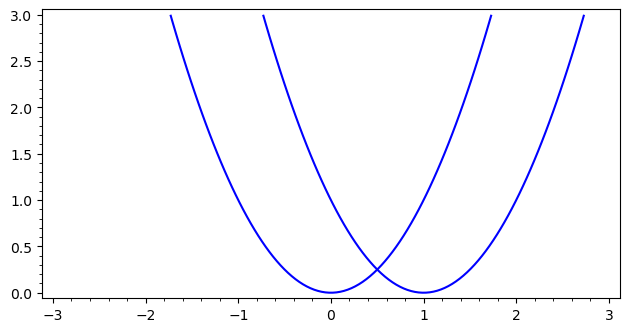
\includegraphics[width=4cm]{transverse-conic-intersection}
\]
Homogenize: \(yz=x^2\) and \(yz=(x-z)^2\).
Claim: the intersection points in the projective plane are 
\[
[x,y,z]=[0,1,0],[2,1,4].
\]
Find intersections: \(x^2=(x-z)^2\), \(0=-2xz+z^2=z(-2x+z)\), so \(z=0\) or \(z=2x\).
If \(z=0\), then \(x=0\), so \([x,y,z]=[0,1,0]\) (remember we can't have all of \(x,y,z\) zero in the projective plane, and if \(y\ne 0\), we can rescale \(y\) to \(y=1\)).
If \(z=2x\), then \(2xy=x^2\), so \(x=0\) or \(2y=x\), so \([x,y,z]=[0,1,0]\) or \([x,y,z]=[2,1,4]\).
Now to compute resultants.
In the affine \(xy\) plane, \(z=1\), we find the intersection point
\[
[x,y,z]=[2,1,4]=[1/2,1/4,1].
\]
The coefficients are:
\[
\begin{array}{ccc}
-x^2&+&y\\
-x^2&,&1\\[10pt]
-(x-1)^2&+&y\\
-(x-1)^2&,&1
\end{array}
\]
So the resultant is
\[
r(x)=
\det
\begin{pmatrix}
-x^2 & -(x-1)^2\\
1&1
\end{pmatrix}=-2x+1,
\]
so the intersection multiplicity at \([x,y,z]=[1/2,1/4,1]\) is \(1\).
At \([x,y,z]=[0,1,0]\), we compute in the affine \((y=1)\) plane, where our curves are \(z=x^2\) and \(z=(x-z)^2=x^2-2xz+z^2\).
\[
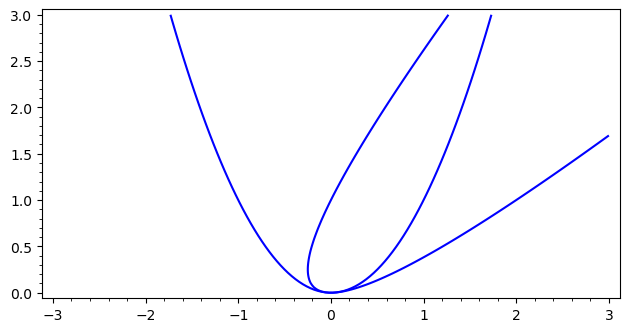
\includegraphics[width=4cm]{triple-conic-intersection}
\]
Expand in \(z\):
\[
0=-x^2+z \text{ and } 0=x^2-(1+2x)z+z^2,
\]
so coefficients
\[
\begin{array}{ccccc}
-x^2&+&z\\
-x^2&,&1\\[10pt]
x^2&-&(1+2x)z&+&z^2\\
x^2&,&-(1+2x)&,&1
\end{array}
\]
The resultant is
\[
r(x)=
\det
\begin{pmatrix}
-x^2&0&x^2\\
1&-x^2&-(1+2x)\\
0&1&1
\end{pmatrix}
=
x^4-2x^3=x^3(x-2),
\]
with roots at \(x=0\) and \(x=2\), corresponding to \([x,y,z]=[0,1,0]\) and \([x,y,z]=[2,1,4]\), with intersection multiplcities \(1,3\).
So these two conics intersect in the affine \(xy\)-plane at \([x,y,z]=[2,1,4]\) transversely (i.e. with intersection multiplicity \(1\)) and then again on the projective line at infinity at \([x,y,z]=[0,1,0]\), with an intersection multiplicity of \(3\).
\end{answer}
\begin{problem}{proj.curves:poles}
Prove that any nonconstant rational function on a curve has poles, perhaps over a finite degree extension field.
\end{problem}
\begin{answer}{proj.curves:poles}
Every nonconstant rational function in the projective plane has poles along a curve, and curves intersect (at points over the algebraic closure of the field, at least), by B\'ezout's theorem.
\end{answer}
\begin{problem}{proj.curves:degree}
Show that the degree of any irreducible plane algebraic curve (i.e. the degree of its equation) is invariant under biregular morphisms of the affine plane.
\end{problem}
\begin{answer}{proj.curves:degree}
The linear functions of the affine plane sit in the algebra of regular functions of the curve.
By B\'ezout's theorem, the linear functions not everywhere vanishing on any component are precisely those regular functions which vanish at a number of points equal to the degree of the curve.
So these functions are preserved, and they span the linear functions.
The linear functions generate the algebra of regular functions, i.e. every regular function is a polynomial expression in the linear functions.
The degree of the curve is the smallest positive degree for which there is a polynomial relation, inside the regular functions, among the linear functions.
\end{answer}
\begin{problem}{counting.intersections:real.circle}
Prove that every real polynomial \(p(x,y)\) in the plane has an even number of real zeroes on any circle in the plane, counting with multiplicity.
\end{problem}
\begin{answer}{counting.intersections:real.circle}
Take any algebraic curve \(C\) of even degree, for example the circle, and any algebraic curve \(B=(0=p(x,y))\) of any degree.
By B\'ezout's theorem, they have an even number of complex intersections, counting multiplicities.
Each intersection point has a complex conjugation intersection point, i.e. with coordinates the complex conjugate, with equal multiplicity.
Each intersection point which is not real is different from its conjugate, so in total the intersection points which are not real arise with an even sum of multiplicities.
So the total number of real intersection points, counting multiplicity, is the total number of complex intersection points minus the total number of complex but not real intersection points, so is a difference of even integers.
\end{answer}

\section{Sage}
Pieter Belmans wrote the following sage code to find the intersection multiplicity of two algebraic curves at a point.
First we find the minimum degree of any term in a polynomial \(f(x)\) of one variable.
\begin{sageblock}
def ldegree(f):
    minimum = infinity
    for (n, m) in f.dict():
        minimum = min(minimum, n)
    return minimum
\end{sageblock}
Given any two polynomials \(b, c\) in two variables, we want to figure out what the two variables are:
\begin{sageblock}
def determine_variables(b, c):
    if len(b.variables()) == 2:
        return b.variables()
    if len(c.variables()) == 2:
        return c.variables()
    if len(b.variables()) == len(c.variables()) == 1:
        if b.variables() == c.variables():
            return (b.variable(0), 0)
        else:
            return (c.variable(0), b.variable(0))
    return (0,0)
\end{sageblock}
Finally, we use our definition of intersection multiplicity, and induction, to compute intersection multiplicities recursively.
\begin{sageblock}
def intersection_multiplicity(b, c, point = (0,0)):
    (x,y) = determine_variables(b, c)
    # translate both curves to origin and calculate it there
    b = b.subs({x:x + point[0], y:y + point[1]})
    c = c.subs({x:x + point[0], y:y + point[1]})
    # if $b(0,0)\neq 0$ or $c(0,0)\neq 0$ they don't intersect in the origin
    if b.subs({x:0, y:0}) != 0 or c.subs({x:0, y:0}) != 0: 
        return 0
    # if $b$ or $c$ are zero they don't intersect properly
    if b == 0 or c == 0: 
        return Infinity
    # we only look at factors of $x$
    f = b.subs({y:0})
    g = c.subs({y:0})
    # $b$ contains a component $y=0$
    if f == 0:
        # $c$ contains a component $y=0$ too, no proper intersection
        if c == 0: 
            return infinity
        # remove common $y^n$ in $b$, count degree of $x$ in $c$ and recurse
        else:
            f = b.quo_rem(y)[0]
            return ldegree(g) + intersection_multiplicity(f, c)
    # $b$ does not contain a component $y=0$
    else:
        # $c$ *does* contain a component $y=0$
        if g == 0:
            g = c.quo_rem(y)[0]
            return ldegree(f) + intersection_multiplicity(b, g)
        # we recurse by removing factors of $x$
        else:
            p, q = f.lc(), g.lc()
            r, s = f.degree(), g.degree()
            # we drop the highest degree term
            if r <= s:
                return intersection_multiplicity(b, p*c - q*x^(s-r)*b)
            else:
                return intersection_multiplicity(q*b - p*x^(r-s)*c, c)
\end{sageblock}
A test run:
\begin{sageblock}
P.<x,y> = PolynomialRing(QQ)
b = P(x^2+y^2)^2+3*x^2*y-y^3
c = P(x^2+y^2)^3-4*x^2*y^2
intersection_multiplicity(b,c)
\end{sageblock}
yields \(\sage{intersection_multiplicity(b,c)}\), the intersection multiplicity at the origin of the curves:
\begin{center}
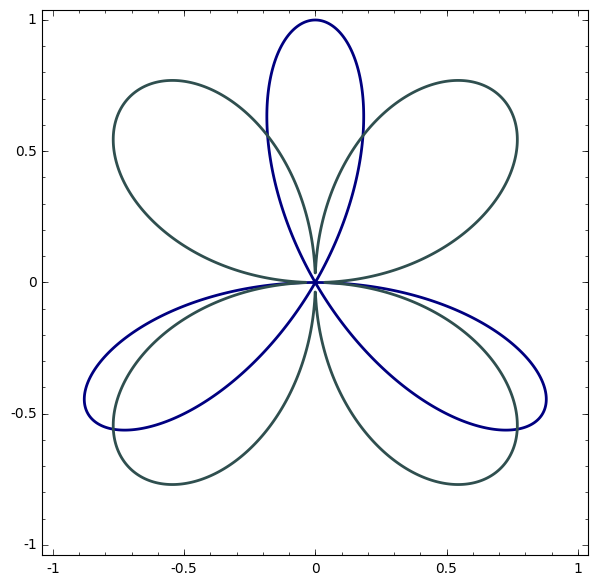
\includegraphics[width=6cm]{curve_intersection}
\end{center}
%p=implicit_plot(b, (x,-1, 1), (y,-1, 1),color="navy",linewidth=2, plot_points=1500)
%q=implicit_plot(c, (x,-1, 1), (y,-1, 1),color="darkslategray",linewidth=2, plot_points=1500)
%show(p+q)
